\documentclass[11pt,a4paper]{scrreprt}

\usepackage[a4paper,top=2.2cm,bottom=2.4cm,left=2.1cm,right=2.1cm]{geometry}
\usepackage[table]{xcolor}
\usepackage{booktabs}
\usepackage{array}
\usepackage{tabularx}
\usepackage{enumitem}
\usepackage{tcolorbox}
\tcbuselibrary{skins,breakable}
\usepackage{tikz}
\usetikzlibrary{positioning,calc,backgrounds}
\usepackage{fontawesome5}
\usepackage{microtype}
\usepackage{titlesec}

%---------------------------------------------------------------
% Palette
%---------------------------------------------------------------
\definecolor{treasurynavy}{RGB}{20,36,60}
\definecolor{treasuryteal}{RGB}{0,121,107}
\definecolor{treasurygold}{RGB}{181,136,66}
\definecolor{treasurygray}{RGB}{243,244,247}
\definecolor{treasurymuted}{RGB}{108,118,132}

\pagestyle{empty}

%---------------------------------------------------------------
% Section styling
%---------------------------------------------------------------
\titleformat{\section}
  {\color{treasurynavy}\Large\bfseries}
  {\thesection}{0.6em}{}
\titlespacing*{\section}{0pt}{1.6em}{0.8em}
\titleformat{\subsection}
  {\color{treasuryteal}\large\bfseries}
  {\thesubsection}{0.5em}{}
\titlespacing*{\subsection}{0pt}{1.2em}{0.5em}

\renewcommand{\arraystretch}{1.15}

%---------------------------------------------------------------
% tcolorbox styles
%---------------------------------------------------------------
\newtcolorbox{policybox}[1]{
  colback=treasurygray,
  colframe=treasurynavy,
  boxrule=0.5pt,
  left=8pt,right=8pt,top=6pt,bottom=6pt,
  arc=1.5pt,
  fonttitle=\bfseries\color{white},
  colbacktitle=treasurynavy,
  title=#1,
  breakable
}

\newtcolorbox{riskbox}[1]{
  colback=white,
  colframe=treasurygold,
  boxrule=0.6pt,
  left=8pt,right=8pt,top=5pt,bottom=5pt,
  arc=1.5pt,
  fonttitle=\bfseries\color{treasurynavy},
  colbacktitle=treasurygray,
  coltitle=treasurynavy,
  title=#1,
  breakable
}

\newcommand{\metric}[2]{%
  {\color{treasurymuted}\small #1}\par
  {\color{treasurynavy}\bfseries\Large #2}%
}

%---------------------------------------------------------------
\begin{document}

%================================================================
% COVER
%================================================================
\begin{tikzpicture}[remember picture,overlay]
  \fill[treasurynavy] (current page.north west) rectangle
       ([yshift=-5.6cm]current page.north east);
  \fill[treasuryteal] ([yshift=-5.6cm]current page.north west) rectangle
       ([yshift=-5.68cm]current page.north east);
\end{tikzpicture}

\vspace*{1.1cm}
{\color{white}
\begin{flushleft}
\hspace{0.2cm}\textcolor{treasurygold}{\rule{2.4cm}{2pt}}\\[0.35cm]
\hspace{0.2cm}{\Large \faLock\ TREASURY \& FINANCE}\\[0.3cm]
\hspace{0.2cm}{\huge\bfseries Corporate Treasury \&\\[2pt] \hspace{0.2cm}Cash Management Plan}\\[0.6cm]
\hspace{0.2cm}{\large Meridian Industrial Group --- Group Treasury Function}
\end{flushleft}
}

\vspace{1.4cm}

\begin{minipage}{0.32\textwidth}
\metric{Reporting Period}{Q3 FY2026}
\end{minipage}\hfill
\begin{minipage}{0.32\textwidth}
\metric{Plan Version}{v4.2 (Board-Approved)}
\end{minipage}\hfill
\begin{minipage}{0.32\textwidth}
\metric{Effective Date}{14 July 2026}
\end{minipage}

\vspace{0.5cm}
\begin{minipage}{0.32\textwidth}
\metric{Prepared By}{Priya Anand, Group Treasurer}
\end{minipage}\hfill
\begin{minipage}{0.32\textwidth}
\metric{Reviewed By}{Marcus Odell, CFO}
\end{minipage}\hfill
\begin{minipage}{0.32\textwidth}
\metric{Classification}{Internal --- Finance Only}
\end{minipage}

\vspace{0.9cm}
\noindent\textcolor{treasurymuted}{\rule{\linewidth}{0.4pt}}

\vspace{0.4cm}
\noindent\textbf{\color{treasurynavy}Purpose of this document.} This plan sets out the
Group's treasury governance, consolidated liquidity position, thirteen-week cash flow
forecast, banking and facility structure, short-term investment policy, and market-risk
controls for the reporting period above. It is the operating reference for the Treasury
Committee and is reissued quarterly or upon material change in the Group's funding
position.

\vspace{1.2cm}

%================================================================
\section{Executive Summary}

Group consolidated cash and equivalents stood at \$164.9M as at 30 June 2026, against a
Board-mandated minimum liquidity buffer of \$60.0M. Net debt reduced by \$8.3M
quarter-on-quarter following the early repayment of the Vertex Distribution equipment
facility. The Group remains within all financial covenants under the Silverbrook Bank
syndicated facility, with the tightest headroom on the interest cover ratio (4.8x against
a 3.5x covenant floor).

\begin{minipage}{0.24\textwidth}
\metric{Available Liquidity}{\$164.9M}
\end{minipage}\hfill
\begin{minipage}{0.24\textwidth}
\metric{Undrawn Facilities}{\$95.0M}
\end{minipage}\hfill
\begin{minipage}{0.24\textwidth}
\metric{Net Debt / EBITDA}{1.9x}
\end{minipage}\hfill
\begin{minipage}{0.24\textwidth}
\metric{Interest Cover}{4.8x}
\end{minipage}
\par
\vspace{0.6cm}

Three items require Treasury Committee attention this quarter: (1) the Synapse Logistics
receivables cycle has extended to 58 days, compressing that entity's operating cash; (2) EUR
exposure on the Nimbus Capital equipment order is 62\% hedged against a 90\% policy target;
and (3) the Ashford Trust revolving facility matures in eight months and should enter
renewal discussions by September.

%================================================================
\section{Treasury Governance \& Policy Objectives}

The treasury function operates under authority delegated by the Board Finance Committee.
Its four standing objectives, in order of priority, are:

\begin{policybox}{Objective Hierarchy}
\begin{enumerate}[leftmargin=1.4em,label=\arabic*.,itemsep=3pt]
  \item \textbf{Solvency} --- maintain sufficient same-day liquidity to meet all obligations
        without recourse to emergency funding.
  \item \textbf{Capital preservation} --- short-term surplus cash is invested only in
        instruments meeting the credit and tenor limits in \S5; return is subordinate to
        principal safety.
  \item \textbf{Cost of funds} --- minimise the Group's weighted average cost of debt
        within the risk limits set by this policy.
  \item \textbf{Risk control} --- hold FX and interest-rate exposure within Board-approved
        hedge ratios (\S6).
\end{enumerate}
\end{policybox}

\vspace{0.4cm}
\noindent Authority limits are tiered by transaction size: the Treasury Manager may
approve payments and intercompany transfers up to \$500K; the Group Treasurer up to \$5M;
amounts above \$5M, or any new banking facility, require joint CFO and Treasury Committee
sign-off. All wire release requires dual authorisation regardless of amount.

%================================================================
\section{Consolidated Cash Position by Entity}

\noindent Balances below are as at close of business 30 June 2026, translated to USD at
the Group's quarter-end reporting rate.

\begin{table}[h!]
\centering
\small
\begin{tabularx}{\textwidth}{@{}Xrrrr@{}}
\toprule
\rowcolor{treasurynavy}
\textcolor{white}{\bfseries Entity} & \textcolor{white}{\bfseries Currency} &
\textcolor{white}{\bfseries Operating Cash} & \textcolor{white}{\bfseries Restricted Cash} &
\textcolor{white}{\bfseries Total Available} \\
\midrule
Nexa Manufacturing Ltd.       & USD & \$38.1M & \$4.5M & \$42.6M \\
\rowcolor{treasurygray}
Synapse Logistics Inc.        & USD & \$16.4M & \$2.5M & \$18.9M \\
Vertex Distribution GmbH      & EUR & \$24.0M & \$3.4M & \$27.4M \\
\rowcolor{treasurygray}
Apex Services Pty Ltd.        & AUD & \$10.1M & \$1.1M & \$11.2M \\
Nimbus Capital (Treasury Ctr.) & USD & \$61.3M & \$3.5M & \$64.8M \\
\midrule
\rowcolor{treasuryteal}
\textcolor{white}{\bfseries Group Total} & & \textcolor{white}{\bfseries \$149.9M} &
\textcolor{white}{\bfseries \$15.0M} & \textcolor{white}{\bfseries \$164.9M} \\
\bottomrule
\end{tabularx}
\caption*{\footnotesize\color{treasurymuted}Restricted cash comprises customer escrow
(Nexa), payroll trust accounts, and cash collateral posted against the Apex bank
guarantee facility.}
\end{table}

\vspace{-0.2cm}
\begin{center}
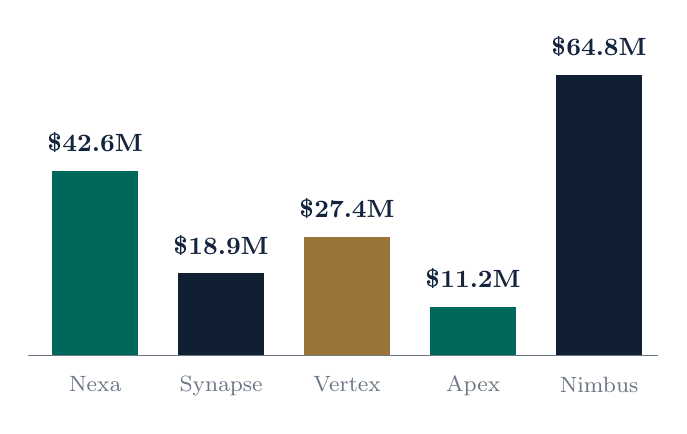
\begin{tikzpicture}
  \def\scaleval{0.055}
  \foreach \name/\val/\xpos/\col in {
    Nexa/42.6/0/treasuryteal,
    Synapse/18.9/1.6/treasurynavy,
    Vertex/27.4/3.2/treasurygold,
    Apex/11.2/4.8/treasuryteal,
    Nimbus/64.8/6.4/treasurynavy}{
    \pgfmathsetmacro{\barheight}{\val*\scaleval}
    \draw[fill=\col!85!black,draw=none] (\xpos,0) rectangle ++(1.1,\barheight);
    \node[anchor=south,font=\small\bfseries,text=treasurynavy] at (\xpos+0.55,\barheight+0.1) {\$\val M};
    \node[anchor=north,font=\footnotesize,text=treasurymuted] at (\xpos+0.55,-0.15) {\name};
  }
  \draw[treasurymuted,thin] (-0.3,0) -- (7.7,0);
\end{tikzpicture}

{\footnotesize\color{treasurymuted}Figure 1. Total available cash by legal
entity (\$M).}
\end{center}

%================================================================
\section{Thirteen-Week Cash Flow Forecast}

The rolling thirteen-week forecast is maintained weekly by each entity controller and
consolidated by Treasury every Monday. The first eight weeks are shown below; weeks 9--13
and the full receipts/disbursements breakdown by category are retained in the Treasury
workbook (Appendix A, not reproduced here).

\begin{table}[h!]
\centering
\small
\begin{tabularx}{\textwidth}{@{}lXrrrr@{}}
\toprule
\rowcolor{treasurynavy}
\textcolor{white}{\bfseries Week} & \textcolor{white}{\bfseries Period Ending} &
\textcolor{white}{\bfseries Receipts} & \textcolor{white}{\bfseries Disbursements} &
\textcolor{white}{\bfseries Net Flow} & \textcolor{white}{\bfseries Ending Balance} \\
\midrule
W1  & 06 Jul 2026 & \$21.4M & \$18.9M & +\$2.5M  & \$167.4M \\
\rowcolor{treasurygray}
W2  & 13 Jul 2026 & \$19.8M & \$23.1M & --\$3.3M & \$164.1M \\
W3  & 20 Jul 2026 & \$24.6M & \$19.5M & +\$5.1M  & \$169.2M \\
\rowcolor{treasurygray}
W4  & 27 Jul 2026 & \$18.2M & \$26.4M & --\$8.2M & \$161.0M \\
W5  & 03 Aug 2026 & \$22.9M & \$20.1M & +\$2.8M  & \$163.8M \\
\rowcolor{treasurygray}
W6  & 10 Aug 2026 & \$17.5M & \$21.7M & --\$4.2M & \$159.6M \\
W7  & 17 Aug 2026 & \$26.1M & \$19.0M & +\$7.1M  & \$166.7M \\
\rowcolor{treasurygray}
W8  & 24 Aug 2026 & \$20.3M & \$24.8M & --\$4.5M & \$162.2M \\
\bottomrule
\end{tabularx}
\end{table}

\noindent The Week 4 and Week 8 outflows reflect quarterly VAT remittance and the
biweekly payroll run coinciding with supplier settlement dates. Forecast ending balance
does not fall below the \$60.0M policy floor at any point in the thirteen-week horizon
under the base case.

%================================================================
\section{Banking Relationships \& Facility Summary}

\begin{table}[h!]
\centering
\small
\begin{tabularx}{\textwidth}{@{}Xlrrrl@{}}
\toprule
\rowcolor{treasurynavy}
\textcolor{white}{\bfseries Bank} & \textcolor{white}{\bfseries Facility} &
\textcolor{white}{\bfseries Limit} & \textcolor{white}{\bfseries Drawn} &
\textcolor{white}{\bfseries Available} & \textcolor{white}{\bfseries Maturity} \\
\midrule
Silverbrook Bank (lead)  & Syndicated RCF        & \$120.0M & \$45.0M & \$75.0M & Mar 2029 \\
\rowcolor{treasurygray}
Ashford Trust Bank       & Revolving Credit       & \$30.0M  & \$18.0M & \$12.0M & Mar 2027 \\
Northgate Financial      & Trade Finance / LC     & \$25.0M  & \$17.0M & \$8.0M  & Dec 2026 \\
\rowcolor{treasurygray}
Cascade Union Bank       & Overdraft (multi-ccy)  & \$10.0M  & \$1.9M  & \$8.1M  & Rolling \\
Harborstone Bank         & Guarantee / Bond Line  & \$8.0M   & \$3.9M  & \$4.1M  & Jun 2028 \\
\midrule
\rowcolor{treasuryteal}
\textcolor{white}{\bfseries Total}& & \textcolor{white}{\bfseries \$193.0M} &
\textcolor{white}{\bfseries \$85.8M} & \textcolor{white}{\bfseries \$107.2M} & \\
\bottomrule
\end{tabularx}
\end{table}

\begin{riskbox}{\faCalendar\ Upcoming Renewal --- Ashford Trust Revolving Credit}
Facility matures March 2027. Policy requires renewal terms to be tabled at least six
months ahead of maturity; Treasury will bring a refinancing proposal to the September
Treasury Committee meeting, including at least two competing indicative term sheets.
\end{riskbox}

%================================================================
\section{Short-Term Investment Policy}

Surplus operating cash beyond the \$60.0M liquidity buffer may be placed in the
instruments below, subject to the counterparty, tenor, and concentration limits shown.
No instrument may be purchased without an investment ticket signed by the Group
Treasurer and logged in the treasury management system.

\begin{table}[h!]
\centering
\small
\begin{tabularx}{\textwidth}{@{}Xccc@{}}
\toprule
\rowcolor{treasurynavy}
\textcolor{white}{\bfseries Instrument} & \textcolor{white}{\bfseries Max \% of Portfolio} &
\textcolor{white}{\bfseries Max Tenor} & \textcolor{white}{\bfseries Min Credit Rating} \\
\midrule
Bank term deposits            & 50\% & 90 days  & A-- \\
\rowcolor{treasurygray}
Government / T-bills          & 100\% & 12 months & AA-- \\
Money market funds (AAA-rated)& 40\% & Overnight & AAA \\
\rowcolor{treasurygray}
Commercial paper (top-tier)   & 20\% & 180 days & A-1 / P-1 \\
Single-counterparty limit     & 25\% & --- & A-- \\
\bottomrule
\end{tabularx}
\end{table}

\noindent As at quarter-end, \$38.4M of surplus cash was placed: \$21.0M in 60-day term
deposits with Silverbrook Bank, \$12.4M in an AAA-rated overnight money market fund, and
\$5.0M in 90-day government T-bills. No single counterparty exceeds the 25\% concentration
limit.

%================================================================
\section{FX \& Interest Rate Risk Management}

\begin{minipage}[t]{0.48\textwidth}
\textbf{\color{treasurynavy}FX exposure.} Transactional exposure arises principally from
Vertex Distribution's EUR-denominated purchasing and Apex Services' AUD payroll. Policy
target is a minimum 90\% hedge ratio on committed exposure over the following two
quarters using forward contracts only; options and structured products require Treasury
Committee pre-approval.
\end{minipage}\hfill
\begin{minipage}[t]{0.48\textwidth}
\textbf{\color{treasurynavy}Interest rate exposure.} 68\% of gross debt is fixed-rate or
swapped to fixed via the interest-rate swap with Silverbrook Bank (notional \$45.0M,
maturing 2029). The remaining floating exposure is monitored monthly against a 150 bps
rate-shock scenario.
\end{minipage}
\par
\vspace{0.5cm}

\begin{riskbox}{\faLock\ Hedge Ratio Below Target --- EUR / Nimbus Equipment Order}
The Nimbus Capital EUR 14.2M equipment order is currently 62\% hedged against the 90\%
policy target. Treasury has requested indicative forward pricing from Silverbrook Bank
and Cascade Union Bank and will close the remaining hedge by 15 August 2026.
\end{riskbox}

%================================================================
\section{Covenant \& Compliance Monitoring}

\begin{table}[h!]
\centering
\small
\begin{tabularx}{\textwidth}{@{}Xccc@{}}
\toprule
\rowcolor{treasurynavy}
\textcolor{white}{\bfseries Covenant (Silverbrook RCF)} & \textcolor{white}{\bfseries Requirement} &
\textcolor{white}{\bfseries Actual} & \textcolor{white}{\bfseries Status} \\
\midrule
Net Debt / EBITDA        & $\leq$ 3.0x & 1.9x & \textcolor{treasuryteal}{\bfseries Pass} \\
\rowcolor{treasurygray}
Interest Cover Ratio     & $\geq$ 3.5x & 4.8x & \textcolor{treasuryteal}{\bfseries Pass} \\
Minimum Liquidity        & $\geq$ \$60.0M & \$164.9M & \textcolor{treasuryteal}{\bfseries Pass} \\
\rowcolor{treasurygray}
Tangible Net Worth       & $\geq$ \$210.0M & \$238.6M & \textcolor{treasuryteal}{\bfseries Pass} \\
\bottomrule
\end{tabularx}
\end{table}

\noindent All covenants tested quarterly under the Silverbrook facility agreement are
satisfied with adequate headroom. The Group Treasurer certifies compliance to the lending
syndicate within ten business days of quarter-end.

%================================================================
\section{Action Items \& Sign-Off}

\begin{policybox}{Actions for the September Treasury Committee}
\begin{enumerate}[leftmargin=1.4em,label=\arabic*.,itemsep=3pt]
  \item Close the outstanding EUR forward hedge on the Nimbus equipment order to reach
        the 90\% policy target (owner: FX Desk, due 15 Aug 2026).
  \item Table refinancing options for the Ashford Trust revolving facility ahead of its
        March 2027 maturity (owner: Group Treasurer, due 30 Sep 2026).
  \item Review Synapse Logistics receivables ageing and agree a collections action plan
        with the entity controller (owner: Treasury Manager, due 08 Aug 2026).
\end{enumerate}
\end{policybox}

\vspace{1.0cm}
\begin{minipage}{0.46\textwidth}
\textcolor{treasurymuted}{\rule{\linewidth}{0.4pt}}\\[2pt]
Priya Anand\\
{\small\color{treasurymuted}Group Treasurer --- Meridian Industrial Group}
\end{minipage}\hfill
\begin{minipage}{0.46\textwidth}
\textcolor{treasurymuted}{\rule{\linewidth}{0.4pt}}\\[2pt]
Marcus Odell\\
{\small\color{treasurymuted}Chief Financial Officer --- Meridian Industrial Group}
\end{minipage}

\end{document}
